\chapter*{\textsc{Introduction}}
\addcontentsline{toc}{chapter}{\textsc{Introduction}}

	\paragraph{}
	L'objectif de cette manipulation est la réalisation de schémas de pilotage élémentaires du robot $Pekee$. Elle se propose de synthétiser et d'analyser des mouvements en ligne droite selon la direction principale du robot. Le mode de commande qu'on utilisera est la réalisation d'un programme C++ $ sous Microsoft Visual C++ $ sur un calculateur fixe qui communique avec le robot par réseau sans fil (Wifi). Trois types de commandes seront étudiées: une commande en boucle ouverte, une commande en boucle fermée; une commande événementielle. Elles seront effectuées successivement en simulation, puis sur le procédé réel. 
	
	\begin{center}
	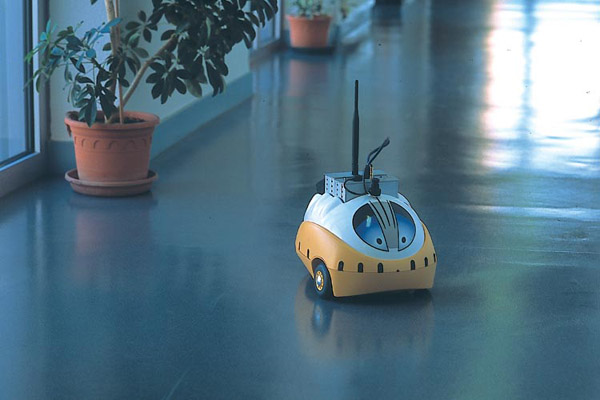
\includegraphics[scale=0.5]{pekee1.jpg}
	\captionof{figure}{\textit{Robot Pekee.\\}}
	\label{fig1} 
	\end{center}   